
\documentclass[11pt]{exam} % https://www.ctan.org/pkg/exam?lang=en

\usepackage[lmargin=1.in,rmargin=1.in,tmargin=1.in,bmargin=1in]{geometry}
\usepackage{setspace}
\usepackage[pdftex]{graphicx}
\usepackage{titling}
\usepackage[
	pdfauthor={Brian Weinstein},
	pdftitle={Homework 4},
	bookmarks=true,
	colorlinks=true,
	linkcolor=blue,
	urlcolor=blue,
	citecolor=blue,
	pdftex,
	linktocpage=true
	]{hyperref}
\usepackage[textsize=tiny]{todonotes}
\usepackage{float}
\setlength\parindent{0pt}
\usepackage{amsmath}
\usepackage{lipsum}


\qformat{\textbf{Problem \thequestion: \thequestiontitle}\quad \hfill}


\pagestyle{headandfoot}
\runningheadrule
\firstpageheader{}{}{}
\runningheader{\thetitle}{\theauthor}{\thedate}
\firstpagefooter{}{\thepage}{}
\runningfooter{}{\thepage}{}


\usepackage{xcolor}
\usepackage{adjustbox}
\usepackage{verbatim}
\definecolor{shadecolor}{rgb}{.9, .9, .9}

\newenvironment{code}%
   {\par\noindent\adjustbox{margin=1ex,bgcolor=shadecolor,margin=0ex \medskipamount}\bgroup\minipage\linewidth\verbatim}%
   {\endverbatim\endminipage\egroup}

\newenvironment{codeSmall}%
   {\par\noindent\adjustbox{margin=1ex,bgcolor=shadecolor,margin=0ex \medskipamount}\bgroup\minipage\linewidth\verbatim\footnotesize}%
   {\endverbatim\endminipage\egroup}


\newcommand{\argmin}[1]{\underset{#1}{\operatorname{argmin}}\;}




\begin{document}


\title{STAT S4240 002, Homework 4}
\author{Brian Weinstein (bmw2148)}
\date{August 13, 2015}
\maketitle



\begin{questions}



\titledquestion{\href{http://www-bcf.usc.edu/~gareth/ISL/}{James} 6.8.1}

\begin{parts}



\part The model obtained through \textit{best subset selection} has the smallest training RSS for $k \leq p$ predictors. This is because best subset selection tests all possible subsets of size $k$ and chooses the one that minimizes the training RSS.
\smallskip

There is a chance that by using \textit{forward stepwise selection} or \textit{backward stepwise selection} we'd end up with the same optimal subset of $k$ predictors (i.e., the one we obtain via best subset selection), but since the $k$-sized subset is dependent on the covariates included in the prior steps in each of these methods, there's no guarantee that this will be the case.

\part Without either valuating each model on a testing set or estimating test error, none among the three models is guaranteed to have the lowest test RSS. These methods only choose the subset that results in the lowest training RSS, which in no way indicates if the model will also result in a low test RSS.

\part

\begin{subparts}

\subpart True. In a model identified by forward stepwise selection, the subset of predictors in a given step (with $k$ predictors) is the base upon which the next predictor is added in the subsequent step (with $k+1$ predictors).

\subpart True. In a model identified by backward stepwise selection, the subset of predictors in a given step (with $k$ predictors) is itself a subset of the predictors used in the previous step (with $k+1$ predictors).

\subpart False. The forward stepwise and backward stepwise models using $k$ predictors are not guaranteed to use the same subset of predictors. As such, once an additional variable is added to the forward stepwise model (or equivalently, once a variable is removed from the backward stepwise model), there's no guarantee that the variables in the $k$-variable backward stepwise model are a subset of the $k+1$-variable forward stepwise model.

\subpart False, with similar reasoning to Part (iii). The $k$ predictors in a forward stepwise model are the predictors that, at each incremental step, kept the error as low as possible. Similarly, the $k+1$ predictors in a backward stepwise model are the predictors at each incremental step that kept the error as low as possible. Since each subset of predictors depends on those used in the previous step, there's no guarantee (although it may happen to be the case) that a set of predictors obtained via forward selection is a subset of those obtained via backward selection.

\subpart False. The set of $k$ predictors chosen in best subset selection are those that keep the error in the $k$-variable model as low as possible. Independently, the set of $k+1$ predictors chosen in best subset are those that keep the error in the $k+1$-variable model as low as possible. There's no guarantee that $k$ of the variables included in the $(k+1)$-variable model are those that minimize the error in the $k$-variable model.


\end{subparts}
 

\end{parts}



\titledquestion{\href{http://www-bcf.usc.edu/~gareth/ISL/}{James} 6.8.3}

Estimating the regression coefficients in a linear regression model via

$$\argmin{\hat{\beta}}\left\{ \sum_{i=1}^{n} \left(    y_i - \beta_0 - \sum_{j=1}^p \beta_j x_{ij} \right) \right\} \quad \text{subject to} \quad \sum_{j=1}^p \left|{\beta_j}\right| \leq s$$

for a given value of $s$.

%is equivalent to estimating the coefficients via
%$$\argmin{\hat{\beta}}\left\{ \sum_{i=1}^{n} \left(    y_i - \beta_0 - \sum_{j=1}^p \beta_j x_{ij} \right)  + \lambda \sum_{j=1}^p \left|{\beta_j}\right|\right\}.$$

As we increase $s$ from 0:

\begin{parts}

\part The training RSS will (\textbf{iv.}) steadily decrease. As we make the constraint on $\sum_{j=1}^p \left|{\beta_j}\right|$ less strict, the limitation on the size of $\hat{\beta}$ disappears and we eventually get the standard ``least residuals'' solution. At $s=0$ we start with only the intercept $\beta_0$ non-zero. As we increase $s$ we allow for additional non-zero coefficients, eventually including all coefficients in the model. With all coefficients included, we minimize the training error (while potentially overfitting).


\part The testing RSS will (\textbf{ii.}) decrease initially, and then eventually start increasing in a U shape. At $s=0$ we start with a highly-biased model with only the intercept $\beta_0$ non-zero. As we increase $s$ we allow for \textit{some} of the $\beta_{j\neq0}$ to take non-zero values (since the constraint is the same as that used in the lasso), which reduces the bias and increases the variance, for an overall drop in RSS. Once we increase $s$ enough, \textit{all} of the $\beta_{j\neq0}$ will take non-zero values and we're left with a model with very low bias, but very high variance, increasing the RSS.

\part The variance will (\textbf{iii.}) steadily increase. The reasoning here is similar to that used in Part (ii): At $s=0$ we start with a very inflexible model, and as we increase $s$ to allow more non-zero coefficients, the model flexibility, and thus our variance, increases.

\part The (squared) bias will (\textbf{iv.}) steadily decrease. The reasoning here is similar to that used in Part (ii): At $s=0$ we start with a highly-biased, very inflexible model with only one coefficient, $\beta_0$. As we increase $s$ to allow more non-zero coefficients, the model flexibility, and thus our squared bias, decreases.

\part The irreducible error will (\textbf{v.}) remain constant. The irreducible error is a function of the data we're given, not the model we choose, so our choice of $s$ has no effect on the size of the irreducible error.

\end{parts}



\titledquestion{\href{http://www-bcf.usc.edu/~gareth/ISL/}{James} 6.8.5}

\begin{parts}

\part asdf

\end{parts}



\titledquestion{\href{http://www-bcf.usc.edu/~gareth/ISL/}{James} 8.4.5}

\begin{parts}

\part asdf

\end{parts}



\end{questions}




%\begin{figure}[H]
%	\centering
%	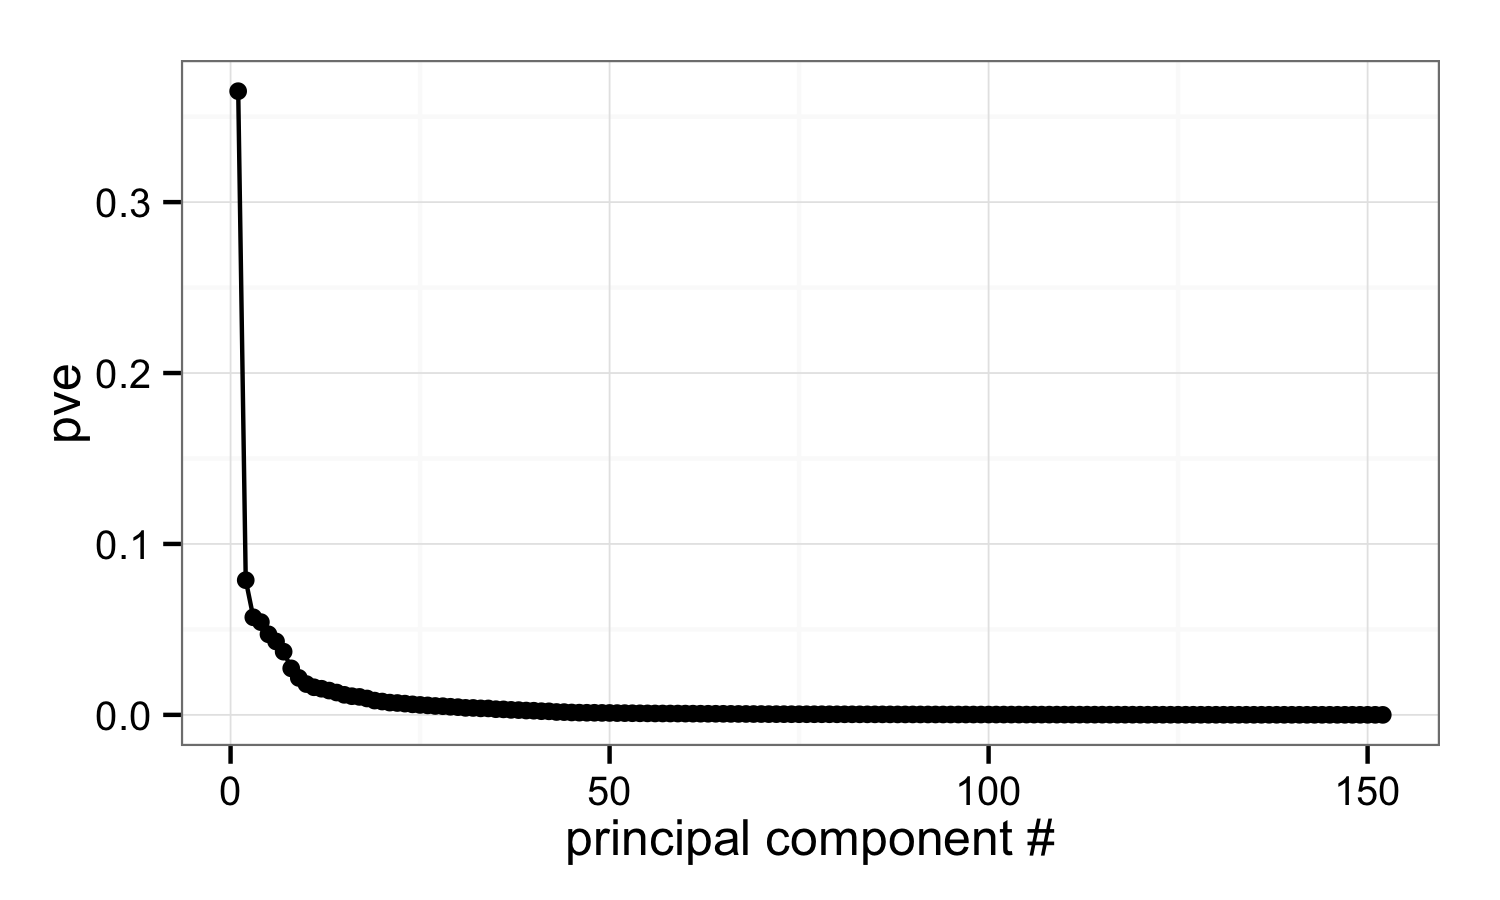
\includegraphics[width=5in]{2c.png}
%	%\caption{}
%	%\label{fig:figName}
%\end{figure}




%\listoftodos

\end{document}